\documentclass[12pt,a4paper]{report}
\usepackage[utf8]{inputenc}
\usepackage[spanish]{babel}
\usepackage{amsmath}
\usepackage{amsfonts}
\usepackage{amssymb}
\usepackage{makeidx}
\usepackage{graphicx}
\usepackage{lmodern}
\usepackage{kpfonts}
\usepackage{fourier}
\usepackage[left=2cm,right=2cm,top=2cm,bottom=2cm]{geometry}
\begin{document}
\section*{Práctica 2\\
Diseño CAD de un robot serial\\
Cinemática de Robots\\
}

Profesor: Morán Garabito Carlos Enrique\\
Integrantes:\\
Medina Rodríguez Francisco Javier\\
Alvarado Galicia Felipe\\
Gutiérrez Muñoz José de Jesús\\
Pasillas González Iván Alejandro\\
Martínez Noyola Moisés Emanuel\\
\\\\\\\\\\\\\\\\\\\\\\\\\\\\\\\\\\\\\\\\\\\\\\\\\\\\\\\\
\\\\\\\\
\section*{Introducción\\}

La definición de un robot serial es la siguiente de acuerdo a la UNIVERSIDAD POLITÉCNICA DE TULANCINGO:\\

\textit{“Los robots seriales, presentan una configuración de eslabones conectados en forma secuencial, empezando por la base hasta el efector final. Cada eslabón de la cadena está unido al anterior mediante articulaciones, ya sean rotacional o prismática, y en todas las articulaciones hay un generador de movimiento o actuador”}
\\\\
Dicho de manera general, este tipo de robot realiza movimientos uno después de otro, el cual es nuestro caso, expuesto en el presente reporte.\\
El diseño del robot es de tipo cilíndrico, mismo que se desarrollará a lo largo del último bloque de formación de la carrera.\\
En esencia, un robot de este tipo es como se muestra en la siguiente imagen:\\\\

$$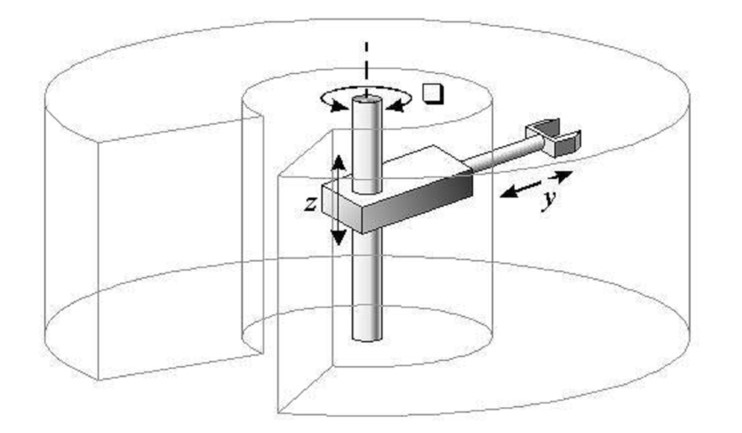
\includegraphics[scale=0.8]{Imagenes/Robot1.jpg}$$\\

$$Figura 1. Robot Cilíndrico$$

La primera articulación es de tipo rotacional, produciendo por consiguiente rotación en torno a la base; el segundo movimiento es de tipo lineal o prismática en el eje Z; finalizando con un movimiento similar, pero en este caso en el eje Y.\\\\\\

\section*{Desarrollo}

En este punto no se cuenta con un análisis completo de los materiales a utilizar, sin embargo, se piensa en emplear metales resistentes al calor debido a la tarea para la cual será diseñado: Soldar cordones.\\
Se ha acorado en el siguiente diseño base para el robot, creyendo que cumple con el mínimo de resistencia considerando materiales metálicos.\\

$$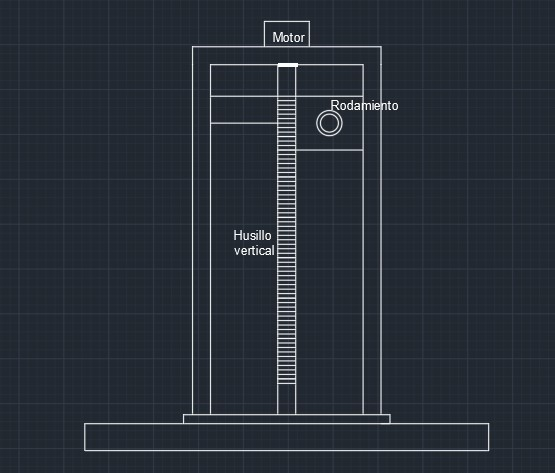
\includegraphics[scale=1]{Imagenes/CADfrontal.jpg}$$

$$Figura 2. Vista frontal del robot$$

Se observa una base, encima de esta la plataforma rotatoria. Dos “Postes” de soporte. En la parte de arriba se colocará el servomotor conectado a un husillo.
Se piensa que en los postes exista una guía de tipo riel.\\

$$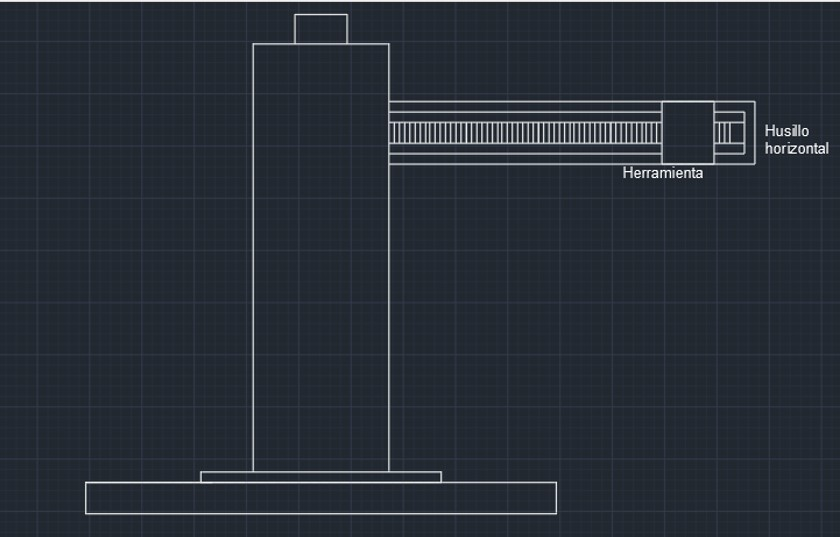
\includegraphics[scale=0.75]{Imagenes/CADLateral.jpg}$$

$$Figura 3. Vista lateral derecha$$\\

Para el movimiento horizontal se ha pensado en el mismo principio que en el vertical: un husillo conectado al motor. \\

Es verdad que un diseño tan básico puede conllevar problemas futuros. Se espera poder solucionarlos de la forma correcta, haciendo un análisis de elementos finitos y selección de materiales.

\section*{Bibliografías}
https://www.milenio.com/opinion/varios-autores/universidad-politecnica-de-tulancingo/resena-historica-de-los-robots-paralelos\\
http://www.udesantiagovirtual.cl/moodle2/mod/book/view.php?id=24911&chapterid=225

\end{document}